\documentclass[10pt, compress]{beamer}

\usetheme{m}
\usepackage{soul}

\usepackage{natbib}
\bibliographystyle{unsrt}
\usepackage{booktabs}
\usepackage[scale=2]{ccicons}
\usepackage{minted}
\usepackage{wrapfig}
\usepackage{enumitem}
\usemintedstyle{trac}
\usepackage{float}
\usepackage{tikz}
\usepackage{standalone}
\usepackage{algorithm}
\usepackage{algorithmicx}
\usepackage[noend]{algpseudocode}
\renewcommand\algorithmicdo{}
\renewcommand\algorithmicthen{}
\newcolumntype{C}[1]{>{\centering\let\newline\\\arraybackslash\hspace{0pt}}m{#1}}

\setbeameroption{show notes}

\begin{document}

\begin{frame}[plain,t]

\begin{wrapfigure}{r}{0.2\textwidth}
\begin{flushright}
\vspace{-2cm}

\includegraphics[width = 10mm]{figures/kth_logo.png}
\end{flushright}
\end{wrapfigure}

\vspace{2cm}

{\large\textbf{Breaking Trivium with Stuck-at-0 Faults}}
\\\rule{7.5cm}{1pt}

\vspace{0.5cm}

{\large Presented by: \textbf{Phillip Gajland}}

\begin{figure}
\includestandalone[width=0.5\textwidth]{figures/modified}
\end{figure}
\end{frame}

\begin{frame}{Today}
\begin{table}
\def\arraystretch{1.2}
\raggedright
\begin{tabular}{r c l}
\textbf{Motivation} &-& Why should you care?\\
\textbf{Background} &-& What do you need to know?\\
\textbf{Trivium} &-& What is it?\\
\textbf{Fault Injection} &-& How does it work?\\
\textbf{Summary} &-& In short?\\
\textbf{Conclusion} &-& And what?
\end{tabular}
\end{table}
\end{frame}

\section{Motivation}

\begin{frame}{Motivation}
\vspace{1cm}
\begin{center}
\centering
{\LARGE\textbf{"23.3 billion IoT devices by 2023"}}\cite{iot}
\end{center}
\end{frame}

\begin{frame}{Motivation}
\begin{itemize}[itemsep=0.5cm]
\item \textbf{23.3 billion IoT devices by 2023:}
\begin{itemize}
\item DDoS attacks e.g. Dyn cyberattack 2016
\end{itemize}
\end{itemize}
\end{frame}

\section{Background}

\begin{frame}{eSTREAM}
\begin{itemize}[itemsep=0.5cm]
\item[$\blacktriangleright$] \textbf{eSTREAM project} - 2004
\begin{itemize}
\item Organised by ECRYPT to \textit{"identify new stream ciphers suitable for widespread adoption"}.
\end{itemize}
\item[$\blacktriangleright$] \textbf{eSTREAM portfolio} - 2008/2011
\begin{table}
\centering
\begin{tabular}{l|l}
Profile 1 (software) & Profile 2 (hardware)\\\hline
HC-128 & Grain\\
Rabiit & MICKEY\\
Salsa20 & Trivium\\
SOSEMANUK & 
\end{tabular}
\end{table}
\end{itemize} 
\end{frame}

\begin{frame}{Trivium}
\begin{columns}
\column{0.5\textwidth}
\begin{itemize}[itemsep=0.5cm]
\item[$\blacktriangleright$] Key: 80-bit key
\item[$\blacktriangleright$] Initialisation Vector: 80-bit
\item[$\blacktriangleright$] Output: $\leq2^{64}-bit$
\item[$\blacktriangleright$] Internal State: 288-bit
\item[$\blacktriangleright$] 3 shift registers:
\begin{itemize}
\item a) 93-bit
\item b) 83-bit
\item c) 111-bit
\end{itemize}
\end{itemize}
\column{0.5\textwidth}
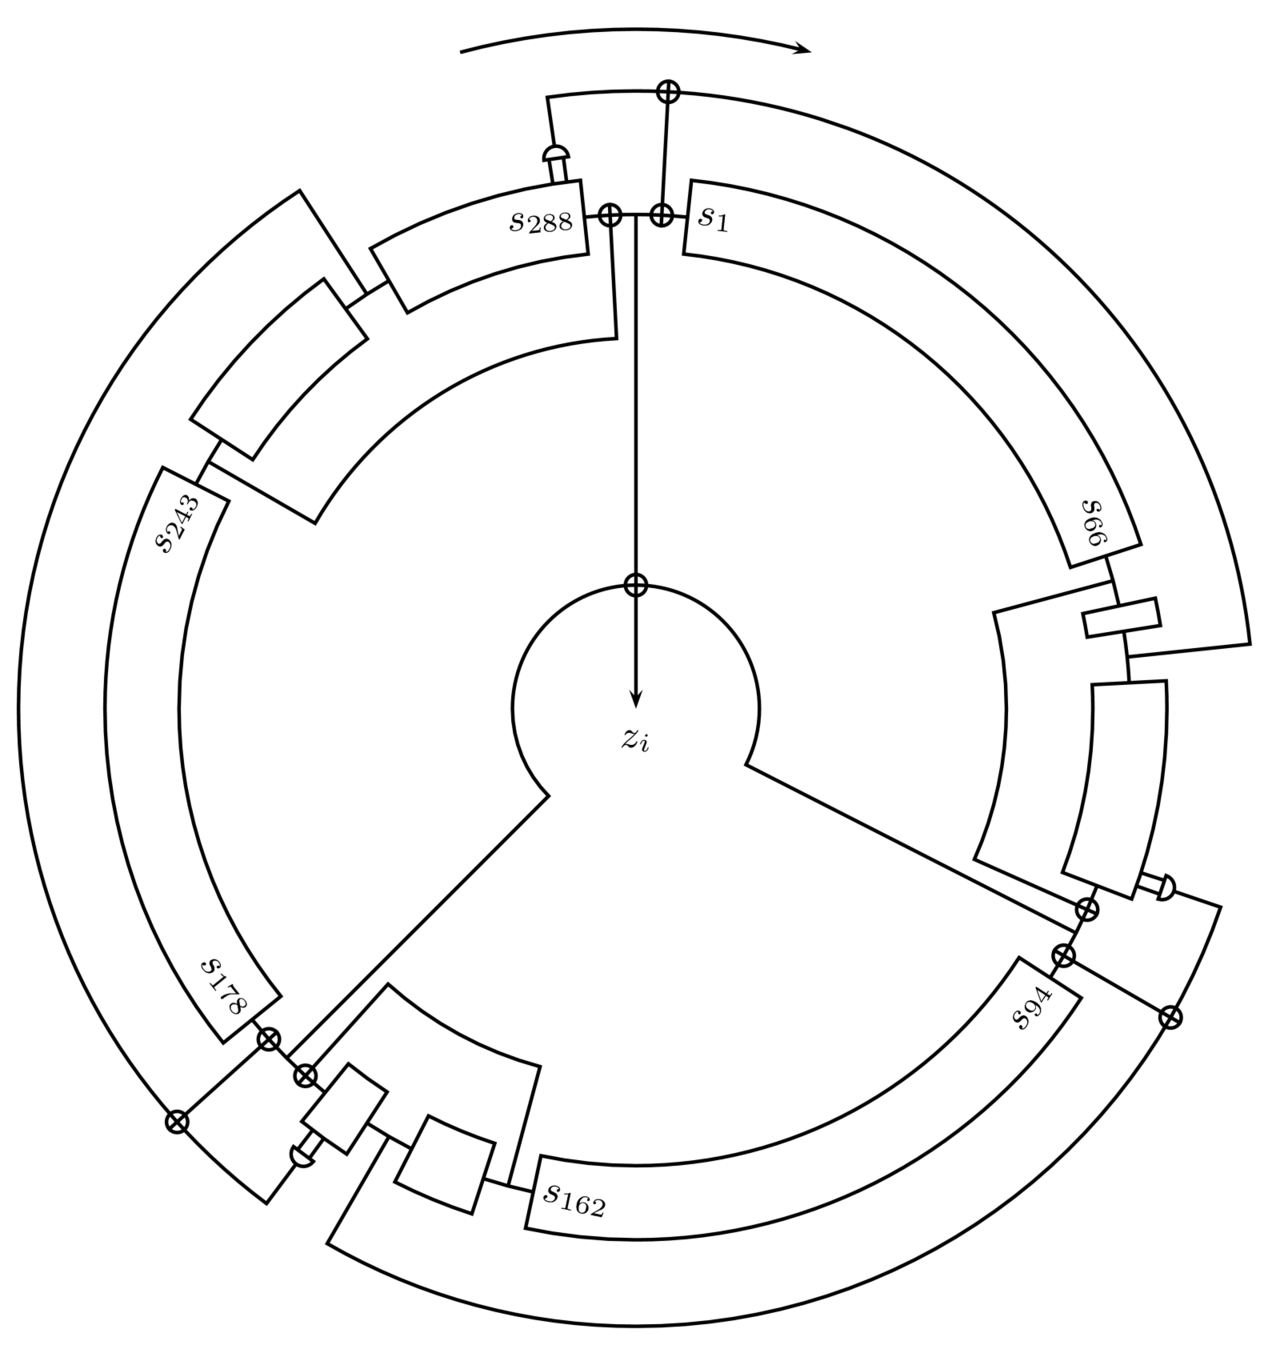
\includegraphics[width=0.9\textwidth]{presentation/figures/round.png}\cite{circle}
\end{columns}
\end{frame}

\begin{frame}{Design}
\begin{figure}
\includestandalone[width=0.95\textwidth]{figures/original}
\end{figure}
\end{frame}

\begin{frame}{Key stream generation}
\begin{center}
\begin{minipage}{\textwidth}
\begin{algorithm}[H]
\begin{algorithmic}[1]
\For{$i=1$ to $N$} \Comment{$N\leq 2^{64}$}
\State $t_1 \gets s_{66} + s_{93}$
\State $t_2 \gets s_{162} + s_{177}$
\State $t_3 \gets s_{243} + s_{288}$
\State
\State $z_i \gets t_1 + t_2 + t_3$
\State
\State $t_1 \gets t_1 + s_{91} \cdot s_{92} + s_{171}$
\State $t_2 \gets t_2 + s_{175} \cdot s_{176} + s_{264}$
\State $t_3 \gets t_3 + s_{286} \cdot s_{287} + s_{69}$
\State
\State $(s_1,s_2,...,s_{93}) \gets (t_3,s_1,...,s_{92})$ \Comment{93 bits}
\State $(s_{94},s_{95},...,s_{177}) \gets (t_1,s_{94},...,s_{176})$ \Comment{83 bits}
\State $(s_{178},s_{179},...,s_{288}) \gets (t_2,s_{178},...,s_{287})$ \Comment{111 bits}
\EndFor
\end{algorithmic}
\end{algorithm}
\end{minipage}
\end{center}
\end{frame}

\begin{frame}{Key and IV setup}
\begin{itemize}
\item[$\blacktriangleright$] Run over 4 full cycles 
\end{itemize}
\begin{center}
\begin{minipage}{\textwidth}
\begin{algorithm}[H]
\begin{algorithmic}[1]
\State $(s_1,s_2,...,s_{93}) \gets (K_1,...,K_{80},0,...,0)$ \Comment{93 bits}
\State $(s_{94},s_{95},...,s_{177}) \gets (IV_1,...,IV_{80},0,...,0)$ \Comment{83 bits}
\State $(s_{178},s_{179},...,s_{288}) \gets (0,...,0,1,1,1)$ \Comment{111 bits}
\State
\For{$i=1$ to $4\cdot288$}
\State $t_1 \gets s_{66} + s_{91} \cdot s_{92} + s_{93} + s_{171}$
\State $t_2 \gets s_{162} + s_{175} \cdot s_{176} + s_{177} + s_{264}$
\State $t_3 \gets s_{243} + s_{286} \cdot s_{287} + s_{288}+ s_{69}$
\State
\State $(s_1,s_2,...,s_{93}) \gets (t_3,s_1,...,s_{92})$ \Comment{93 bits}
\State $(s_{94},s_{95},...,s_{177}) \gets (t_1,s_{94},...,s_{176})$ \Comment{83 bits}
\State $(s_{178},s_{179},...,s_{288}) \gets (t_2,s_{178},...,s_{287})$ \Comment{111 bits}
\EndFor
\end{algorithmic}
\end{algorithm}
\end{minipage}
\end{center}
\end{frame}

\section{Fault Injection}

\begin{frame}{Fault Injection}
\begin{figure}
\includestandalone[width=0.95\textwidth]{figures/modified}
\end{figure}
\end{frame}

\begin{frame}{Key stream generation}
\begin{center}
\begin{minipage}{\textwidth}
\begin{algorithm}[H]
\begin{algorithmic}[1]
\For{$i=1$ to $N$} \Comment{$N\leq 2^{64}$}
\State $t_1 \gets s_{66} + s_{93}$
\State $t_2 \gets s_{162} + s_{177}$
\State $t_3 \gets s_{243} + s_{288}$
\State
\State $z_i \gets t_1 + t_2 + t_3$
\State
\State $t_1 \gets t_1 + s_{171}$
\State $t_2 \gets t_2 + s_{264}$
\State $t_3 \gets t_3 + s_{69}$
\State
\State $(s_1,s_2,...,s_{93}) \gets (t_3,s_1,...,s_{92})$ \Comment{93 bits}
\State $(s_{94},s_{95},...,s_{177}) \gets (t_1,s_{94},...,s_{176})$ \Comment{83 bits}
\State $(s_{178},s_{179},...,s_{288}) \gets (t_2,s_{178},...,s_{287})$ \Comment{111 bits}
\EndFor
\end{algorithmic}
\end{algorithm}
\end{minipage}
\end{center}
\end{frame}

\begin{frame}{Key and IV setup}
\begin{itemize}
\item[$\blacktriangleright$] Run over 4 full cycles 
\end{itemize}
\begin{center}
\begin{minipage}{\textwidth}
\begin{algorithm}[H]
\begin{algorithmic}[1]
\State $(s_1,s_2,...,s_{93}) \gets (K_1,...,K_{80},0,...,0)$ \Comment{93 bits}
\State $(s_{94},s_{95},...,s_{177}) \gets (IV_1,...,IV_{80},0,...,0)$ \Comment{83 bits}
\State $(s_{178},s_{179},...,s_{288}) \gets (0,...,0,1,1,1)$ \Comment{111 bits}
\State
\For{$i=1$ to $4\cdot288$}
\State $t_1 \gets s_{66} + s_{93} + s_{171}$
\State $t_2 \gets s_{162} + s_{177} + s_{264}$
\State $t_3 \gets s_{243} + s_{288}+ s_{69}$
\State
\State $(s_1,s_2,...,s_{93}) \gets (t_3,s_1,...,s_{92})$ \Comment{93 bits}
\State $(s_{94},s_{95},...,s_{177}) \gets (t_1,s_{94},...,s_{176})$ \Comment{83 bits}
\State $(s_{178},s_{179},...,s_{288}) \gets (t_2,s_{178},...,s_{287})$ \Comment{111 bits}
\EndFor
\end{algorithmic}
\end{algorithm}
\end{minipage}
\end{center}
\end{frame}





\section{END}

\plain{}{Questions?}

\begin{frame}{Acknowledgements}
\begin{table}
\centering
\begin{tabular}{l l}
Latex Beamer: & \url{github.com/matze/mtheme}\\
& \\
& \\
GitHub: & \url{github.com/GaPhil/trivium}
\end{tabular}
\end{table}
\end{frame}

\begin{frame}{Sources}
\bibliography{bibl}
\nocite{*}    
\end{frame}

\end{document}